\section{Opsi Respons}
\label{sec:opsi}

Empat opsi mitigasi dibandingkan dengan simulasi PowerShift (cara kerja di Bagian~\ref{sec:inovasi}). Seluruh angka keuangan adalah selisih kumulatif 2026-2040 terhadap baseline phase down, yaitu PLTU pensiun di akhir PPA atau umur desain dan PLTS atap tumbuh mengikuti tren dengan aturan sekarang. Hasilnya diringkas pada Tabel~\ref{tab:preset} dan Gambar~\ref{fig:preset}.

\begin{table}[H]
\centering
\caption{Hasil simulasi empat opsi, kumulatif 2026-2040 terhadap baseline phase down}
\label{tab:preset}
\small
\resizebox{\textwidth}{!}{\begin{tabular}{lrrrr}
\toprule
Indikator & PLTS atap saja & Pensiun dini saja & Paket Cirebon-1 & Paket seimbang \\
\midrule
Neraca PLN (Rp T) & -120,0 & 2,1 & -117,8 & 1,4 \\
Neraca negara, PLN + APBN (Rp T) & -132,6 & 2,1 & -130,5 & 3,5 \\
Dana luar ETM/JETP (Rp T) & 0,0 & 3,1 & 3,1 & 14,7 \\
Hemat tagihan pelanggan (Rp T) & 162,3 & 0,0 & 162,3 & 21,6 \\
CO$_2$ dihindari (Mt) & 158,3 & -0,9 & 157,5 & 21,4 \\
Kematian dini dihindari & 7.473 & 4.436 & 11.909 & 8.921 \\
Nilai kesehatan (Rp T) & 86,9 & 51,6 & 138,5 & 103,7 \\
PLTS atap 2040 (GWp) & 19,1 & 4,0 & 19,1 & 5,5 \\
Pembangkit pengganti (MW) & 0 & 660 & 660 & 2.580 \\
Kenaikan BPP maks. (Rp/kWh) & 37,0 & 0,0 & 36,1 & 3,0 \\
\bottomrule
\end{tabular}
}
\sumber{simulasi PowerShift, parameter pada Lampiran~\ref{app:asumsi}}
\end{table}

\subsection{Phase Down di Akhir PPA}

Opsi ini adalah kebijakan yang berjalan sekarang dan menjadi baseline. Kelebihannya, tidak ada biaya kompensasi dan risiko hukum terhadap kontrak IPP. Keterbatasannya, sebagian besar PLTU Jawa-Bali baru pensiun setelah 2040, sehingga emisi dan dampak kesehatan sekitar 8.700 kematian per tahun (Tabel~\ref{tab:pltu}) terus berlangsung.

\subsection{Penetrasi PLTS Atap}

Opsi ini mengembalikan nilai ekspor PLTS atap ke 65\%, menaikkan kuota Jawa-Bali menjadi 1.500 MW per tahun, mewajibkan 100 MW per tahun di gedung pemerintah, dan mengalihkan 5\% subsidi listrik untuk PLTS atap pelanggan 450/900 VA. Kapasitas PLTS atap pada 2040 naik dari 4,0 menjadi 19,1 GWp, menghindari 158 juta ton CO$_2$ dan sekitar 7.500 kematian dini. Keterbatasannya, neraca PLN memburuk sekitar Rp120 triliun karena pendapatan ritel berpindah ke pemilik PLTS atap, dan BPP naik hingga 37,0 Rp/kWh. Hasil ini mengonfirmasi H1 dan menjelaskan mengapa PLN menahan PLTS atap.

\subsection{Pensiun Dini PLTU}

Opsi ini memensiunkan Cirebon-1 pada 2035, sesuai kesepakatan dengan ADB \parencite{B-ADB-CIREBON}, dengan 75\% kompensasi dari dana luar. Kelebihannya, PLN berhenti membayar kapasitas IPP sehingga neracanya membaik Rp2,1 triliun, dan sekitar 4.400 kematian dini dihindari. Keterbatasannya, karena jendela oversupply sudah tertutup pada 2035, PLN tetap membutuhkan 660 MW pembangkit pengganti. Emisi juga praktis tidak turun karena energi Cirebon-1 dipasok PLTU lain.

\subsection{Paket Berpasangan}

Opsi ini menggabungkan kedua opsi sebelumnya (Paket Cirebon-1). Neraca PLN membaik sekitar Rp2,2 triliun dibanding PLTS atap saja, sehingga H2 terbukti, tetapi perbaikannya kecil dibanding kerugian dari pendapatan ritel. Manfaat kesehatannya paling besar, sekitar 11.900 kematian dini dihindari atau setara Rp138,5 triliun.

\subsection{Perbandingan Opsi}

\begin{figure}[H]
\centering
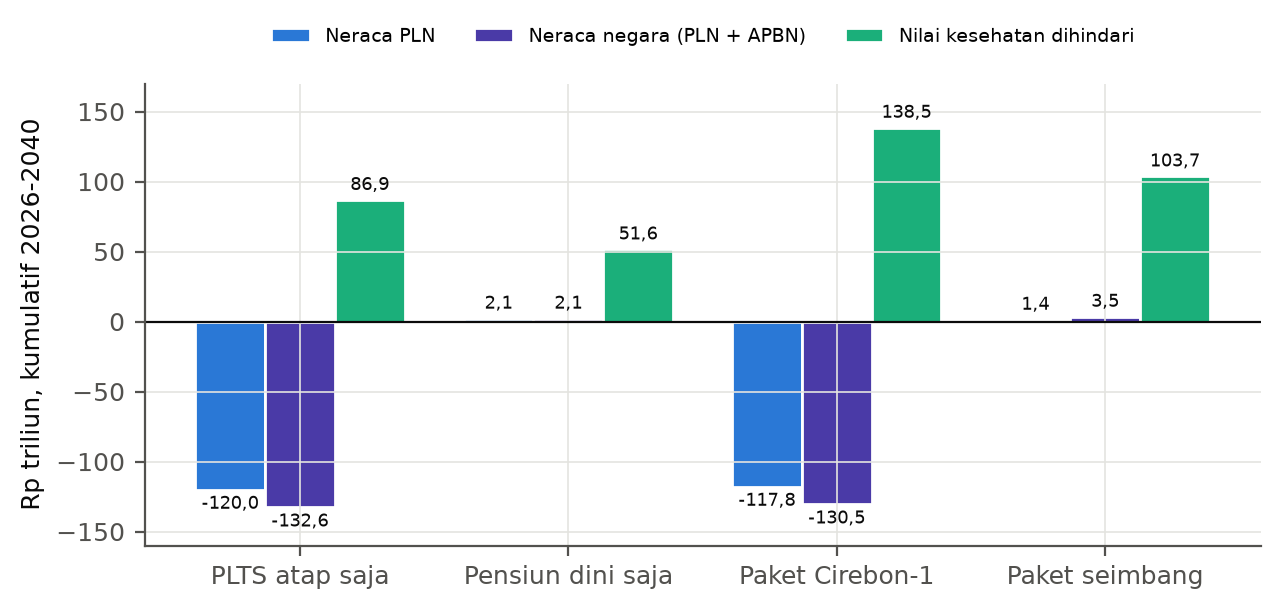
\includegraphics[width=\textwidth]{neraca_preset}
\caption{Neraca PLN, neraca negara, dan nilai kesehatan per opsi (kumulatif 2026-2040)}
\label{fig:preset}
\sumber{simulasi PowerShift}
\end{figure}

Gambar~\ref{fig:preset} menunjukkan pola yang konsisten: setiap opsi yang menambah PLTS atap secara besar membebani PLN dan APBN, sementara nilai kesehatannya berpindah ke masyarakat. Pensiun dini IPP dengan dana luar menguntungkan PLN, tetapi manfaat emisinya baru muncul bila energinya digantikan energi bersih. Karena itu dibutuhkan alat untuk mencari kombinasi yang seimbang, yang dijelaskan pada bagian berikut.
